% SPDX-License-Identifier: CC-BY-4.0
% Copyright (c) 2026 Jonathan Yantis. Research draft; not submitted.
\documentclass[11pt,letterpaper]{article}
\usepackage[margin=0.85in]{geometry}
\usepackage[T1]{fontenc}
\usepackage{mathptmx,amsmath,amssymb,booktabs,array,ragged2e,xcolor,microtype,xurl,hyperref,fancyhdr,longtable,tikz}
\usetikzlibrary{arrows.meta,positioning}
\definecolor{studyblue}{RGB}{39,83,109}
\hypersetup{colorlinks=true,urlcolor=studyblue,citecolor=studyblue,linkcolor=black,pdfauthor={Jonathan Yantis},pdftitle={A Shared Time Base for Bluetooth Timecode Ecosystems: PToB Architecture, Compatibility Boundaries, and a Validation Programme}}
\setlength{\parindent}{1em}\setlength{\parskip}{3pt}\setlength{\headheight}{14pt}\setlength{\emergencystretch}{2em}
\widowpenalty=10000\clubpenalty=10000
\renewcommand{\floatpagefraction}{0.8}\renewcommand{\topfraction}{0.9}\renewcommand{\textfraction}{0.1}
\pagestyle{fancy}\fancyhf{}\fancyhead[L]{\small PToB and Bluetooth Timecode}\fancyhead[R]{\small Research draft, 22 October 2026}\fancyfoot[C]{\small\thepage}
\newcolumntype{L}[1]{>{\RaggedRight\arraybackslash}p{#1}}
\newcommand{\ns}{\,\mathrm{ns}}\newcommand{\ms}{\,\mathrm{ms}}\newcommand{\ppm}{\,\mathrm{ppm}}
\newcommand{\code}[1]{\texttt{#1}}
\begin{document}
\title{\vspace{-1.2em}A Shared Time Base for\\Bluetooth Timecode Ecosystems\\[5pt]\large PToB Architecture, Compatibility Boundaries,\\and a Validation Programme}
\author{Jonathan Yantis}
\date{22 October 2026\\\small Research draft; not submitted or peer reviewed}
\maketitle
\begin{abstract}
Bluetooth timecode products already serve cameras, audio recorders and capture applications, but a common radio bearer does not make their interfaces interoperable. This paper investigates Precision Time over BLE (PToB) as a prospective shared time base beneath multiple ecosystem-specific compatibility layers. The proposed contribution is a transport-independent contract binding a continuous clock coordinate to source ancestry, event identity, validity, uncertainty and an exact rational frame or sample mapping. Separate presentation adapters would supply supported Bluetooth timecode interfaces, app timestamps, or optional linear and MIDI timecode outputs. Manufacturer documentation establishes existing integrations in the AirGlu BT and Tentacle ecosystems and distinct control, jam and output mechanisms in Ambient and Deity products; it does not establish PToB compatibility or an openly implementable universal Bluetooth timecode protocol. Historical PToB observations motivate the clock-distribution research but do not measure a timecode receiver, sensor exposure, audio sample clock or calibrated UTC output. We retain those populations and their availability limits separately, derive frame-boundary and holdover constraints, and specify falsifiable validation gates from offline arithmetic through independent recorded-event measurement. A practical initial deployment would combine a native application adapter with a qualified conventional timecode output before pursuing permission-dependent vendor integrations. No adapter, firmware change, new hardware experiment or standards-conformance result is claimed.
\end{abstract}
\noindent\small Copyright \copyright\ 2026 Jonathan Yantis. Original manuscript and figures: \href{https://creativecommons.org/licenses/by/4.0/}{CC BY 4.0}. Executable verification code: MIT.\normalsize

\section{Introduction}
A small production may combine mirrorless cameras, body-worn audio recorders, phone capture and a workstation. Each can record a timecode label, yet the label may have arrived by a different path: a wired linear timecode input, a Bluetooth receiver, a phone application, or a local generator jammed at the beginning of the day. A shared label convention alone does not specify the oscillator, the physical event being labelled, or what happens when synchronization disappears. An integration can appear successful on the display while leaving a recording offset, long-term drift or an unreported outage.

PToB explores distribution of source-scoped time over Bluetooth Low Energy periodic advertising, using physical-event timestamp association and causal clock maps. Its existing research considers rooted timing paths, relays, source validity and a USB-to-macOS application-clock extension \cite{viability,usb}. These mechanisms motivate a question beyond sensor timestamping: could a shared PToB time base support several timecode ecosystems without requiring each endpoint to speak the PToB mesh protocol?

Our hypothesis is conditional. If an adapter can obtain a valid PToB clock, convert it into the exact coordinate required by an endpoint, and control or characterize the endpoint's timing interface, then several such adapters could share a common source. The compatibility layer would preserve the semantic differences between interfaces rather than translate only the visible digits. A radio clock with small conditional phase residuals is insufficient evidence that these additional conditions hold.

This paper contributes (i) a primary-source compatibility survey with explicit implementation boundaries; (ii) a proposed time, quality and event contract; (iii) rational frame/sample mapping and an error model that retains unknown endpoint terms; and (iv) a staged, measurable adoption and validation programme. This is an architectural research draft, not a new wire specification. The literature access date is 22 October 2026. The latest PToB physical evidence discussed is the separate 19 October pilot. No new timing measurement, commercial-device integration, permission agreement or hardware operation was performed for this manuscript.

\section{What a shared time base must mean}
\subsection{Four different services}
We distinguish four requirements that are often grouped under ``sync.'' First, \emph{timecode agreement} associates a frame or recording location with an address such as hours, minutes, seconds and frames. Second, \emph{event-time agreement} estimates when an identified event occurred on a common coordinate. Third, \emph{frequency agreement} controls the long-term rate of a media clock. Fourth, \emph{phase alignment} controls the placement of sensor exposure, video synchronization or audio sampling edges.

Delivering timecode does not by itself guarantee genlock or word-clock control. A particular device may derive additional synchronization from its timecode input, but that is a separate, device-specific capability to verify. Likewise, recording an address in a file does not establish that the address describes exposure start, exposure midpoint, the first audio sample or the instant at which an app callback ran. The endpoint contract must name that observation point.

SMPTE ST 12-1 defines time and control code representations and signal interfaces; it also discusses rate and phase relationships \cite{st12}. SMPTE ST 2059-1 defines deterministic interface-signal alignment to an epoch and associated generation procedures \cite{st2059}. The present proposal does not establish conformance to either standard. It uses their distinction between a time address and a generated interface signal to avoid assigning a physical timing guarantee to metadata alone.

\subsection{Bluetooth bearer, protocol and endpoint behavior}
Bluetooth is the common bearer in the surveyed products. It does not establish a shared application protocol, public service UUID, role, packet timing convention or vendor authorization. A central that controls several boxes has different scheduling and connection requirements from a receiver of a periodic timing train. Support for ordinary BLE connections does not establish controller support for PToB's periodic-advertising and timestamping path.

An adapter must declare whether it supplies a running time reference, performs a one-time jam, configures another generator, or only reads status. A jam transfers an initial condition; the endpoint subsequently depends on its own clock and its documented resynchronization behavior. A running connection can still conceal receiver-side filtering and extrapolation. BLE packets that describe time are not a transport for the camera's video or the recorder's audio. Media transport and capture control remain separate systems.

\section{Documented ecosystem boundaries}\label{sec:compatibility}
\subsection{Survey method and claim limits}
We inspected manufacturer product specifications, operating manuals and official integration guidance. Table~\ref{tab:ecosystems} records the positive capability each source supports, then states the additional work a PToB integration would require. It is a dated, selected survey, not an exhaustive supported-device list. Commercial features, firmware revisions and operating-system behavior can change. A named integration is evidence for that documented pair and configuration, not evidence that PToB can impersonate either product.

No complete public vendor BLE wire protocol or generally available implementation SDK was established by the reviewed sources. This finding does not prove that none exists; a vendor may provide a partner interface or a separate licensed programme. An adapter targeting those interfaces therefore remains contingent on verified technical access, applicable permissions and device testing. This manuscript supplies no protocol reconstruction and makes no claim about reverse-engineering rights.

\begin{table}[htbp]\centering\small
\caption{Documented mechanisms and proposed integration boundaries. Every PToB adapter in this table is unimplemented and unqualified. ``Candidate'' is a research route, not a compatibility assertion.}\label{tab:ecosystems}
\begin{tabular}{@{}L{0.15\linewidth}L{0.42\linewidth}L{0.36\linewidth}@{}}\toprule
Ecosystem & Documented existing capability & PToB candidate and unresolved dependency\\\midrule
Atomos / AirGlu BT & UltraSync Blue serves compatible Bluetooth timecode clients; Nikon Z6III and Zoom F3 manuals describe reception \cite{atomos,nikon,zoom}. & Vendor-supported transmitter or approved bridge; protocol access, supported rates, client behavior and per-device calibration unknown.\\\addlinespace
Tentacle & SYNC E supports Bluetooth sync/control and LTC; official guidance documents Blackmagic Camera app use, and Epic documents its capture workflow \cite{tentacle,blackmagic,epic}. & Native app partnership or supported generator ingress; reproducing a Tentacle Bluetooth source is not established.\\\addlinespace
Ambient & LockitBT supplies Bluetooth remote control and timecode information to compatible third-party devices; ACN provides inter-Lockit synchronization \cite{ambient}. & Supported LTC/MIDI external-master path or vendor-approved Bluetooth integration; named third-party compatibility not inferred.\\\addlinespace
Deity & Sidus Audio supports Bluetooth sync/control of TC-1 boxes; boxes provide local timecode outputs and separate wireless master sync \cite{deityguide}. & Supported external jam input or approved control integration; direct Bluetooth delivery to arbitrary cameras not documented here.\\\addlinespace
Native PToB app & Source-scoped timing and USB-to-macOS application clocks have separate research evidence \cite{viability,usb}. & New application API and recording integration; no existing SMPTE output or commercial receiver interoperability result.\\\bottomrule
\end{tabular}
\end{table}

\subsection{AirGlu BT: direct reception with device-specific limits}
Atomos specifies six Bluetooth clients in UltraSync Blue server mode and a free-running oscillator figure of $0.5\ppm$ \cite{atomos}. Those are product specifications, not a PToB capacity limit or an end-to-end time-error measurement. Its RF-locked zero-ppm wording does not imply zero delivered phase error. The Nikon Z6III guide describes AirGlu BT setup and an important loss case: a current shot continues recording timecode after the wireless link is lost, while the display eventually reports loss \cite{nikon}. Withdrawing an adapter's transmissions therefore cannot be assumed to invalidate consumer metadata.

The Zoom F3 manual requires a BTA-1 or other specified wireless adapter for UltraSync BLUE reception and says the F3 cannot simultaneously connect to F3 Control and UltraSync BLUE \cite{zoom}. Panasonic's S1II product documentation identifies Bluetooth timecode synchronization with UltraSync BLUE \cite{panasonic}; Tascam's DR-10L Pro documentation identifies the optional AK-BT1 path \cite{tascam}. These examples establish a useful cross-device ecosystem while demonstrating why exact model, accessory, mode and firmware belong in a test matrix. They do not establish a generic Bluetooth timecode input available on every camera or recorder.

\subsection{Tentacle: generator control and application integration}
Tentacle specifies a $0.2\ppm$ TCXO and less than one frame drift in 24 hours for SYNC E, alongside Bluetooth setup/synchronization and LTC operation \cite{tentacle}. Its Blackmagic Camera guidance describes selecting a Tentacle source in the application and gives platform-specific rate instructions \cite{blackmagic}. Those instructions motivate testing the actual rate interpretation rather than trusting a rounded UI label. Epic's iOS capture documentation provides an official application context for external timecode \cite{epic}. These integrations make an application-facing route credible; they do not show that a new PToB peripheral can be selected as a Tentacle generator.

\subsection{Ambient and Deity: preserve the control/output distinction}
Ambient documents a Bluetooth interface for remote control and transmission of timecode information to compatible third-party devices, while its own ACN connects Lockit units. Its external-master mode accepts LTC or computer MIDI timecode \cite{ambient}. A research gateway could investigate those documented ingress paths before requesting a direct Bluetooth integration. The stated $0.1\ppm$ calibration and C-Jam drift descriptions concern oscillator/network behavior, not a calibrated third-party BLE receiver error \cite{ambientaccuracy}.

Deity documents Sidus Audio Bluetooth synchronization and control separately from TC-1 wireless master sync and cable input/output modes \cite{deityguide}. Its product page specifies $\pm0.5\ppm$ \cite{deity}. The sources do not establish a direct Bluetooth timecode input for an arbitrary camera. These distinctions matter: controlling a generator can be useful compatibility work without being equivalent to sending timecode directly into the recording device.

\section{Architecture: one source coordinate, several adapters}\label{sec:architecture}
\subsection{Separate clock distribution from presentation}
Figure~\ref{fig:architecture} proposes a common boundary between the PToB timing plane and endpoint presentation. The timing plane supplies a causal map from a local counter to an identified source coordinate. A media-coordinate layer assigns exact frame/sample positions. An adapter then implements one approved endpoint interface. Each branch has its own admission, capacity, delay and validation record. No endpoint has to join the mesh merely to receive a compatible output.

\begin{figure}[htbp]\centering
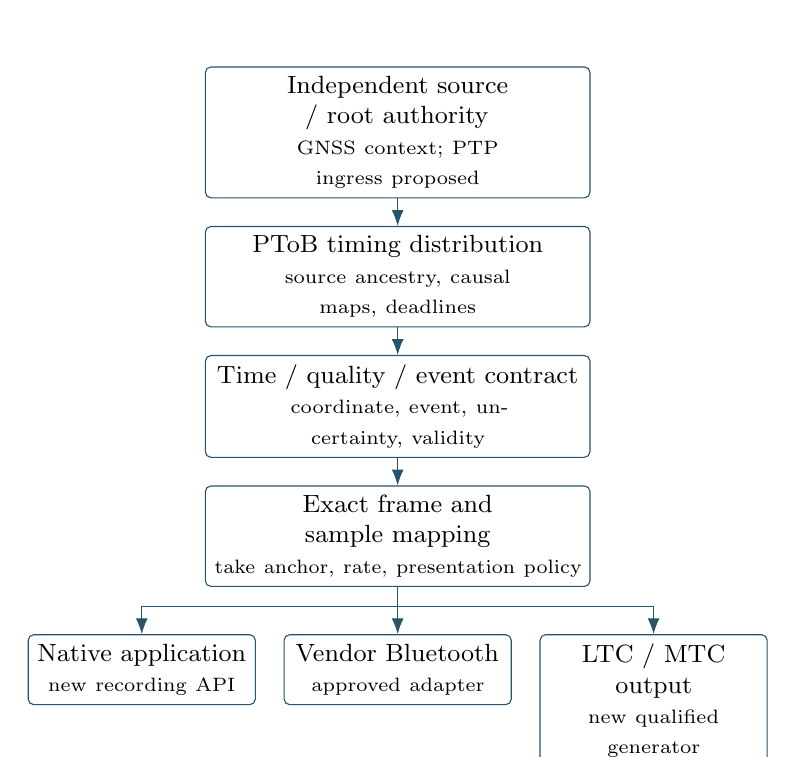
\begin{tikzpicture}[font=\small,box/.style={draw=studyblue,rounded corners=2pt,align=center,minimum height=0.64cm,text width=4.65cm},smallbox/.style={box,text width=2.65cm},arr/.style={-{Latex[length=2mm]},draw=studyblue}]
\node[box] (source) {Independent source / root authority\\\scriptsize GNSS context; PTP ingress proposed};
\node[box,below=0.35cm of source] (mesh) {PToB timing distribution\\\scriptsize source ancestry, causal maps, deadlines};
\node[box,below=0.35cm of mesh] (contract) {Time / quality / event contract\\\scriptsize coordinate, event, uncertainty, validity};
\node[box,below=0.35cm of contract] (frame) {Exact frame and sample mapping\\\scriptsize take anchor, rate, presentation policy};
\node[smallbox,below=0.6cm of frame,xshift=-3.25cm] (native) {Native application\\\scriptsize new recording API};
\node[smallbox,below=0.6cm of frame] (vendor) {Vendor Bluetooth\\\scriptsize approved adapter};
\node[smallbox,below=0.6cm of frame,xshift=3.25cm] (legacy) {LTC / MTC output\\\scriptsize new qualified generator};
\draw[arr] (source)--(mesh);\draw[arr] (mesh)--(contract);\draw[arr] (contract)--(frame);
\draw[arr] (frame.south)--++(0,-0.25)-|(native.north);
\draw[arr] (frame)--(vendor);
\draw[arr] (frame.south)--++(0,-0.25)-|(legacy.north);
\end{tikzpicture}
\caption{Proposed architecture. Lower media and compatibility layers are new work. PTP ingress is a proposal in the viability paper, not an operating bridge. Arrows represent logical dependencies, not one demonstrated deployment.}\label{fig:architecture}
\end{figure}

This split supports gradual adoption. A native application can consume richer quality metadata than a legacy timecode input. A qualified LTC output can use existing wired inputs without claiming a vendor Bluetooth implementation. A future partner adapter can translate to an approved ecosystem while sharing the same source and take anchor. These are alternative presentation paths over a common coordinate, not a claim that one packet format already serves every product.

\subsection{Proposed time and quality record}
Table~\ref{tab:contract} defines a semantic contract rather than a byte layout. Fields can be bound by a session descriptor instead of repeated in every message, provided the binding is unambiguous and survives recording/replay. Unknown uncertainty or civil-time association is represented explicitly; a missing bound is not zero.

\begin{table}[htbp]\centering\small
\caption{Minimum proposed contract at the adapter boundary. None of these additions changes current PToB firmware in this work.}\label{tab:contract}
\begin{tabular}{@{}L{0.25\linewidth}L{0.69\linewidth}@{}}\toprule
Field group & Required interpretation\\\midrule
Coordinate & Timescale identifier, epoch definition, integer seconds plus exact fraction or fixed tick unit, and era/range. Root-relative time remains distinct from TAI or UTC.\\\addlinespace
Source scope & Root identity, root incarnation/source epoch, selected ancestry, bridge identity, local boot/counter epoch and map generation. Preserve original source age.\\\addlinespace
Event & Event identifier and counter value; meaning such as radio capture, scheduled output transition, exposure midpoint or first sample; retrospective estimate versus scheduled future event.\\\addlinespace
Quality & State, last admissible source observation, validity deadline, map age, holdover model, known bias/calibration identifier, and uncertainty type with observation point.\\\addlinespace
Media mapping & Take/mapping identifier, continuous anchor, frame or sample ordinal at anchor, exact rate numerator/denominator, label mode, day/rollover and leap policy.\\\addlinespace
Presentation & Endpoint model/firmware, interface/profile version, effective event time, expected device action, output delay and calibration scope, acknowledgement and loss behavior.\\\bottomrule
\end{tabular}
\end{table}

A clock estimate can be expressed abstractly as
\begin{equation}
 \widehat{T}_g(c)=T_g+a_g(c-c_g),\qquad c\in\mathcal{V}_g,
 \label{eq:clock}
\end{equation}
where $g$ identifies an immutable map, $c$ is the local counter and $\mathcal{V}_g$ is its permitted validity interval. A delivered or scheduled event uses a map available before the relevant deadline. A retrospective fit can annotate a recording later, but must not be reported as a real-time clock that was delivered then. The selected endpoint policy can impose a shorter interval than the underlying map permits.

The proposed states are \code{UNAVAILABLE}, \code{ACQUIRING}, \code{TRACKING}, \code{HOLDOVER} and \code{DISCONTINUITY}. TRACKING means admitted recent observations under a declared policy, not a particular accuracy certification. HOLDOVER requires a finite deadline and a stated growth model. An unknown error bound may be accepted for exploratory logging but cannot satisfy a bounded-error output requirement. DISCONTINUITY invalidates queued mappings until a new segment/anchor is established. These states are adapter-design requirements; existing firmware state names and permissions remain authoritative for current operation.

\subsection{Ancestry, multiple devices and loop prevention}
Each output retains the original source ancestry even if an intermediate box regenerates a signal. A gateway must not ingest its own downstream timecode through another interface and advertise it as independent time. Candidate ingress is rejected when its ancestry contains the local bridge, when its origin is ambiguous, or when the required source authority cannot be established. A jammed commercial box is not an independent reference merely because its output is well formed.

Several endpoint adapters may share one root while using different rates. They still need a common take anchor and explicit event definitions; a 25 fps camera and a $30000/1001$ fps camera will not have equal frame ordinals. A root or epoch change fences stale queued packets and calibration/mapping state whose scope no longer applies. Seamless continuation is a separate, measurable policy, not an automatic consequence of receiving another valid source. Group authentication protects membership and freshness under its threat model; it does not measure source correctness or prevent all compromised-member behavior. PToB authentication and provenance are not automatically preserved by a legacy or vendor timecode format. A sidecar records the bridge's observations, and must distinguish them from proof of what the endpoint actually received; no end-to-end authenticated-time guarantee follows from the upstream authentication alone.

\section{Continuous time, civil presentation and media coordinates}\label{sec:mapping}
\subsection{Timescale and epoch are explicit design choices}
TAI provides a continuous reference coordinate, while UTC introduces leap-second relationships described by BIPM \cite{bipm}. A future PToB media contract could adopt elapsed SI seconds from 1 January 1970 00:00:00 TAI, consistent with the epoch in ST 2059-1 \cite{st2059}. This is a proposed extension. Current PToB root-relative clock mapping and POSIX-style UTC association must not be relabelled as an implemented TAI service. Choosing the same epoch is also insufficient to implement ST 2059 signal generation or its PTP profile.

Conversion to UTC requires an identified, valid TAI--UTC relationship and a versioned leap policy. A timestamp should indicate whether civil association is known, unknown or extrapolated. During an inserted leap second, POSIX-style encodings may repeat or suppress a civil representation; the media ordinal can remain continuous. Smearing, if supported at all, needs a distinct timescale identifier and declared transformation. Time zone, daylight-saving changes and a human-readable time-of-day display must not silently change the continuous take coordinate.

For a long take, day rollover is presentation metadata. The system keeps an unbounded or sufficiently wide take ordinal and a segment/day identifier even when a legacy display wraps at 24 hours. A daily jam, leap conversion or source restart that changes the label-to-coordinate mapping creates a recorded mapping transition. It must not silently rewrite the meaning of previously recorded frames.

\subsection{Exact rational frame and sample arithmetic}
Let a declared common anchor $T_0$ correspond to frame ordinal $N_0$, with exact rate $r=p/q$ frames per SI second. For the convention that an instant belongs to the frame interval beginning at or before it,
\begin{align}
 N(T)&=N_0+\left\lfloor (T-T_0)\frac{p}{q}\right\rfloor,\label{eq:frame}\\
 T_N&=T_0+(N-N_0)\frac{q}{p}.\label{eq:boundary}
\end{align}
An adapter scheduling frame $N$ uses $T_N$; an adapter timestamping an actual capture evaluates the captured event. A receive callback timestamp is not substituted for the capture event without a characterized transfer relation. Negative differences require mathematical floor division, not truncation toward zero. Integer products must be range-checked; an exact remainder accumulator avoids repeated rounded period additions.

For nanosecond differences $\Delta n$, Equation~\ref{eq:frame} evaluates the integer quotient $\lfloor\Delta n p/(10^9q)\rfloor$. Common intended fractional rates include $24000/1001$, $30000/1001$ and $60000/1001$; UI strings ``23.98,'' ``29.97'' and ``59.94'' require a profile-defined interpretation. Literal decimal $29.97$ is not exactly $30000/1001$. At $30000/1001$, a frame lasts $1001/30000$ s, or $33.366\overline{6}\ms$. At $60000/1001$, it lasts $16.683\overline{3}\ms$. These are arithmetic facts, not measured endpoint accuracy.

An audio sample coordinate is defined similarly:
\begin{equation}
 S(T)=S_0+\lfloor (T-T_0)f_s\rfloor,\label{eq:sample}
\end{equation}
with exact sample rate $f_s$. At 48 kHz and $30000/1001$ fps the mean is $8008/5=1601.6$ samples per frame; assigning 1602 samples to every frame would accumulate error. An exact five-frame interval contains 8008 nominal samples. These coordinates describe intended relationships. They do not discipline a recorder's physical ADC clock or imply that its samples actually occur at those ideal instants.

\subsection{Labels and drop-frame numbering}
We retain the continuous ordinal through all label conversions. For nominal 30-count drop-frame labels at $30000/1001$ fps, the labels 00 and 01 are omitted at the start of each minute except every tenth minute; frames themselves are not discarded. For a valid label $(h,m,s,f)$ within a nominal day, let $M=60h+m$. The ordinal from the start of that label day is
\begin{equation}
 N_{\rm DF}=30(3600h+60m+s)+f-2\left(M-\left\lfloor M/10\right\rfloor\right).
 \label{eq:df}
\end{equation}
Skipped labels are invalid inputs. Thus \code{00:00:59;29} is followed by \code{00:01:00;02}, while the tenth-minute transition uses \code{00:10:00;00}. The semicolon is a display convention used here. At 23.976 there is no drop-frame mode defined by this proposal. A $60000/1001$ coordinate is supported mathematically, but an adapter's high-rate time address, frame-pair/field convention and transport representation require an explicit applicable profile; one must not infer a vendor's 59.94 support from the rational mapping alone \cite{st12}.

The nominal 29.97 DF label day has $2{,}589{,}408$ frames. At exact rate $30000/1001$, it lasts $86{,}399.9136$ SI seconds, $86.4\ms$ less than 86,400 seconds. Drop-frame labels therefore do not equal exact civil elapsed time indefinitely. A continuous-take policy can retain ordinals while a civil-day policy records explicit jams or mapping changes. ST 2059-1 provides specific time-address-generation procedures and jam/jump metadata; Equation~\ref{eq:df} alone is not that full procedure \cite{st2059}. The paper's offline verifier checks the analytical examples and all minute transitions in one nominal DF day.

\subsection{Boundary uncertainty and event identity}
Even a small clock error can yield adjacent labels when an event lies near a frame boundary. If a justified event interval is $[\widehat T-u,\widehat T+u]$, define
\begin{equation}
 N^- = N(\widehat T-u),\qquad N^+=N(\widehat T+u).\label{eq:ambiguous}
\end{equation}
For this conservative closed-interval test, a unique frame is supported only if $N^-=N^+$. For example, an event estimated $50\ns$ before a boundary with a $100\ns$ bound spans two candidate frames. A low RMS is neither this bound nor a guarantee that all queries return identical labels. Independent queries made at different physical instants can legitimately straddle a boundary even with perfect clocks.

A richer application stores the continuous event estimate, uncertainty semantics, mapping ID and possible ordinal interval. A legacy endpoint that requires one label needs a declared tie/rounding policy and an ambiguity sidecar; selecting one value cannot erase the uncertainty. Measuring capture alignment therefore requires independently identifying the same optical or electrical event across devices, not comparing two asynchronously sampled displays.

\section{Adapter behavior and multi-device feasibility}\label{sec:adapters}
\subsection{Effective event time and presentation latency}
A future native API should support both \emph{timestamp this captured counter/event} and \emph{schedule this identified boundary}. A device-specific Bluetooth adapter must determine what its packet's time means: the transmission event, a future effective boundary, a local clock reading, or a complete time address interpreted by receiver firmware. If the interface supplies no event association, transport/application delay becomes an unknown error term. Sending the most recent label at callback time does not solve that ambiguity.

Scheduling in advance can reduce sensitivity to variable packet arrival only when the receiver has a usable clock model and an agreed effective-time semantics. An acknowledgement can prove acceptance without proving physical execution. Calibration must bind to device model, firmware, mode, rate, port, signal level and observation point. A fixed latency correction is insufficient when internal buffering or exposure behavior changes. A separate recording delay can exist after a correctly generated timecode transition.

\subsection{Optional LTC and MTC outputs}
A PToB-disciplined LTC generator could provide a conventional compatibility path for equipment with documented input support. It needs deterministic waveform timing, correct labels and flags, specified electrical levels and independent transition/decoder measurements. DAC or audio-interface output adds buffering, sample-clock and restart behavior that must be characterized. A correct decoded address does not establish correctly phased transitions. No LTC generator or pin output is implemented in this work.

MIDI Time Code offers Quarter Frame and Full message types \cite{midi}. A future MTC adapter must implement the appropriate message semantics, receiver interpretation and transport timing; writing a full label to MIDI is not equivalent to aligning media capture. MIDI message format does not establish BLE-MIDI support or bounded Bluetooth latency. These output paths are deliberately separate from vendor BLE protocol emulation and from genlock or audio clock synthesis.

\subsection{Connection, radio and controller budgets}
PToB reception and commercial connected-client service may compete for radio time, controller buffers and host scheduling. Coexistence of periodic advertising reception, scanning and several legacy connections requires an actual controller/stack capability record. The number of endpoints in a product specification is not portable to a different bridge. Table~\ref{tab:capacity} identifies the resources to measure before making a multi-device claim.

\begin{table}[htbp]\centering\small
\caption{Multi-device feasibility questions. No row is resolved by a BLE bitrate alone.}\label{tab:capacity}
\begin{tabular}{@{}L{0.23\linewidth}L{0.71\linewidth}@{}}\toprule
Resource & Required characterization\\\midrule
Radio/controller & Supported simultaneous roles, connection intervals, scan windows, periodic train retention, collision/loss and missed event capture under coexistence.\\\addlinespace
Endpoint fan-out & Maximum admitted clients per interface; reconnect storms, pairing persistence and simultaneous control-app restrictions.\\\addlinespace
Time freshness & Worst source/map age after all adapters are active; original deadlines continue through bridge queues.\\\addlinespace
Scheduling & Per-endpoint preparation/effective-time deadline, queue bounds, CPU work, output clock stability and backpressure.\\\addlinespace
Operations & Identity binding, configuration version, battery replacement, rate changes, firmware upgrades, status visibility and exportable recording audit.\\\bottomrule
\end{tabular}
\end{table}

As an explicitly hypothetical payload calculation, a 64-byte time/quality record delivered ten times per second to six separate clients is $64\times10\times6=3840$ payload bytes/s. This excludes framing, acknowledgements, connection events, security, retries and all PToB timing traffic. The small payload demonstrates only that media-volume transport is unnecessary. It does not establish schedulability, latency, energy use or six-client operation on any PToB target. Separate radios or multiple gateways might be justified if coexistence or permissions impose incompatible roles. A dual-radio bridge also needs a measured counter-transfer relation and its own uncertainty budget; adding a radio does not remove the timing boundary.

\subsection{Loss, stale time and legacy metadata}
At the adapter boundary, source expiry cancels pending qualified outputs whose deadlines no longer hold. Endpoint behavior is a separate state machine: it may stop recording timecode, free-run, retain the previous jam or hide its loss indication. The Nikon example in Section~\ref{sec:compatibility} demonstrates why output suppression alone cannot guarantee downstream invalidity.

A proposed sidecar records source scope, mapping version and intervals of TRACKING, HOLDOVER, unavailable or unknown endpoint state against recording/take identifiers. A consumer that cannot carry uncertainty or expiry needs a visible operator warning and an editorially useful audit. If neither firmware integration nor a sidecar can communicate the distinction, the system must report that downstream validity is unobservable. ``Last connected'' is not evidence of qualified time throughout a take.

\section{What the existing PToB evidence supports}\label{sec:evidence}
\subsection{Historical one-relay phase and coverage}
The 12 October V14 collection contains a prospective two-link path, GM to one RC to a leaf. It reports $62.503871\ns$ RMS including bias and $191\ns$ maximum absolute phase over 436 reference-valid causal samples. Conservative usable coverage is $436/602=72.425\%$. The 602 nominal boundaries comprise 436 valid samples, 65 reference-invalid causal samples, three reference-valid edges with expired maps and 98 unobserved opportunities. The all-causal population of 501 samples, including the 65 reference-invalid observations, has approximately $3.929\ms$ RMS and $19.753\ms$ maximum. These failures and gaps remain in the public collection \cite{v14}.

The measured quantity is a causal software map evaluated at local physical PPS observations, using fractional-second phase and a previously fixed per-link normalization. It is not calibrated UTC, absolute whole-second correctness, independently generated LTC, sensor timing or a measured output pin. Original calibration inputs and raw captures are not all available for independent reconstruction. The result motivates studying a timing substrate; it does not qualify any compatibility adapter.

\subsection{USB/macOS delivery is a separate population}
The 17 October supplement selects every observation in a fixed concurrent 180-second shared-USB-bus RC/DC window. For the BLE-derived RC path, causal RX prediction RMS is $190.049810\ns$ over 5054 scored observations; delivered chrony time minus its own fine input has $325.544636\ns$ RMS over 145 same-instant comparisons. At 177 status samples, 147 show delivery and 30 withholding. Those are three different populations. The window is after acquisition, and a separate failed first-minute RC attempt with no valid UTC replies remains disclosed. The two extended trials were unfinished at the cutoff \cite{usb}.

Delivered-minus-input agreement shares a source; it is not an independent UTC comparison. The bus was shared, and the RC and direct paths used separate physical source chains. These observations cannot establish a controlled transport ranking or a camera-facing Bluetooth result. The existing host extension is useful architectural experience for a native application API, not evidence that a recording framework timestamps captures correctly.

\subsection{Awake HOLD research retains six runs}
The 19 October power-scheduling paper reports six separate awake PC117 runs. Eligible local PPS fractional-phase RMS ranges from $80.259267\ns$ to $2173.739217\ns$ across the six runs, with 1400 eligible recorded HOLD edges in total. Its BLE metric uses a different observation population and an inherited provisional $+10543\ns$ normalization. Only 42 of 120 training windows refreshed the fit; sparse BLE observation coverage and the short post-turnover interval remain explicit \cite{power}.

The radio and precision counter stayed awake. These results establish neither sleep energy savings nor qualified long-duration holdover. The six runs are not pooled into one precision figure, and their best case is not transferred to commercial receivers. Across all three evidence collections, protocol/profile, firmware, instrumentation, populations, correction assumptions and validity policy differ. The present paper introduces no combined performance distribution.

\section{Error budgets without invented bounds}\label{sec:error}
\subsection{Observation point determines the budget}
For a specified physical event on endpoint $i$, a useful bookkeeping model is
\begin{equation}
 e_i=b_{\rm source}+b_{{\rm path},i}+b_{{\rm output},i}+b_{{\rm capture},i}
       +\eta_{{\rm map},i}+\eta_{{\rm transport},i}+\eta_{{\rm hold},i}.
 \label{eq:error}
\end{equation}
The $b$ terms represent potentially systematic offsets; the $\eta$ terms denote variable components whose distributions need measurement. Their decomposition is an experimental aid, not proof that the terms are independent or separately identifiable. If justified absolute bounds exist, a conservative bound can add them. If only standard uncertainties are justified, covariance matters:
\begin{equation}
 u_i^2=\sum_j u_{ij}^2+2\sum_{j<k}\operatorname{Cov}(e_{ij},e_{ik}).\label{eq:cov}
\end{equation}
Unknown systematic terms prohibit a complete numerical accuracy claim. Conditional map RMS cannot be substituted for every term. Source errors common to two devices can cancel in a relative comparison while remaining in absolute UTC error. Conversely, local output and capture offsets can survive despite excellent common-clock agreement.

\begin{table}[htbp]\centering\small
\caption{Current status of the proposed end-to-end budget. ``Unknown'' is retained rather than assigned a convenient small value.}\label{tab:budget}
\begin{tabular}{@{}L{0.25\linewidth}L{0.39\linewidth}L{0.30\linewidth}@{}}\toprule
Term & Evidence or design information & Remaining measurement\\\midrule
Source / UTC & Root-relative timing and source association research & Independent absolute reference, leap/whole-second correctness\\\addlinespace
PToB map / path & Separate conditional phase, prediction and coverage populations & New deployment calibration and complete availability\\\addlinespace
Adapter / Bluetooth & Proposed semantics and documented commercial workflows & Packet-event meaning, delay, jitter, coexistence, receiver behavior\\\addlinespace
Output / recording & Proposed LTC/MTC/application paths & Physical transition, exposure/sample event and file metadata relation\\\addlinespace
Holdover / failure & Explicit finite policy required & Device drift, temperature, link loss, restart and stale-state propagation\\\bottomrule
\end{tabular}
\end{table}

\subsection{Oscillator drift is a different quantity}
For an illustrative constant fractional rate error $\epsilon$, elapsed phase drift after $\tau$ seconds is
\begin{equation}
 |\Delta t|=|\epsilon|\tau.\label{eq:drift}
\end{equation}
At 24 hours, $0.5\ppm$, $0.2\ppm$ and $0.1\ppm$ correspond arithmetically to $43.2\ms$, $17.28\ms$ and $8.64\ms$, respectively. These examples use the magnitudes in the cited oscillator specifications; they are not new product measurements, device-pair errors or Bluetooth receive delays. Initial jam error, changing temperature, steering, calibration and correlations are absent from this model. Vendor ``less than one frame'' statements also depend on rate, operating conditions and resynchronization, so they must not be reverse-converted into a calibrated BLE phase bound.

If an application permits total magnitude $B$, has a justified initial bound $E_0$ and a justified constant holdover rate bound $\rho$, then a simplified deadline is
\begin{equation}
 \tau_{\max}\leq (B-E_0)/\rho,\qquad B>E_0,\quad\rho>0.\label{eq:hold}
\end{equation}
For a hypothetical $1\ms$ budget, $0.2\ms$ initial bound and $0.5\ppm$ holdover bound, the maximum is 1600 s, approximately 26.7 minutes. This is not an acceptance interval for any surveyed device. If $E_0$ or $\rho$ is unknown, this calculation cannot qualify the outage period. A probabilistic objective needs a separate distribution and confidence statement.

Frame granularity, oscillator drift and observed map phase are therefore different axes. No numerical superiority ratio between PToB and a commercial Bluetooth timecode system follows from comparing these quantities. A useful comparison must identify the same event, reference, population, duration and acceptance criterion.

\section{A falsifiable validation programme}\label{sec:validation}
\subsection{Stage 0: semantic and arithmetic conformance}
Before connecting equipment, freeze the adapter contract, source/epoch interpretation, exact rate table, supported label modes and loss policy. Exercise negative time differences, overflow, counter wrap, cold boot, source incarnation change and stale queued data. Use independent reference vectors at all minute/tenth-minute/hour/day transitions, including invalid DF labels and the nominal DF day mismatch. Test a leap insertion, unknown offset, explicit smear identifier and a daily mapping change without rewriting a running take. Test interval-valued events on both sides of a frame boundary.

The included standard-library verifier covers the paper's arithmetic examples, DF day transitions and edition identity. It is not a running adapter, vendor protocol test or firmware acceptance suite. A later implementation must add independent serialization and behavioral tests rather than treating the paper equations as executable conformance by themselves.

\subsection{Stage 1: independently observe a native output}
Implement one native application interface or a deterministic LTC output in an isolated development branch. Fix the requirement before collecting data: observation point, maximum error or statistical target, minimum availability, warm-up limit, expected outage behavior and confidence/reporting method. Identify reference instrumentation and its calibration/uncertainty independently of the clock under test.

For LTC, capture actual electrical transitions and decode every label against independently observed time. For an application, record an electrical/optical stimulus observed by both the reference instrument and the capture device. Report raw transition/event error, decoded-address error, fixed offset, drift, distribution tails and the count of invalid, undecodable or missing events. A loopback that shares the same local clock is a diagnostic, not an independent absolute reference. Retain signed errors and avoid retrospective detrending of a real-time claim.

\subsection{Stage 2: qualify one specific compatibility path}
Acquire a supported interface and any necessary vendor cooperation, then freeze model, serial alias, firmware, accessory, rate and mode. First establish the commercial source/receiver baseline using the same instrumentation, event and reporting rules intended for the PToB path. Then substitute the candidate adapter without changing the acceptance criteria. Preserve unsuccessful pairing, rejected configurations, missed outputs and failed restarts. An app setting or successful connection counts as functional setup, not timing acceptance.

Test metadata in the recorded files alongside actual exposure or sample events. Sweep recording modes and frame rates, confirm whether a fixed delay correction remains valid, and test battery replacement, reboot and source change during and between takes. For a jam path, separate initial jam error, free-running drift and re-jam discontinuity. For a running path, measure receiver extrapolation and stale output after both radio loss and upstream-source expiry.

\subsection{Stage 3: multi-device duration, mobility and interference}
An initial research matrix should include one endpoint per accepted interface, then the intended maximum population. Predeclare cold-start repetitions and hours-long runs sufficient to reveal drift; a practical first campaign could use 30 cold starts per configuration and three eight-hour runs, followed by a 24-hour run that crosses a label-day boundary. These are proposed sample sizes, not completed tests or a general reliability proof. Preserve all attempts, explain stopping rules and report confidence limits appropriate to the observed population.

Include controlled temperature ranges within equipment ratings, moving receivers, obstructions, crowded 2.4 GHz traffic, simultaneous phone control, reconnect storms and battery transitions. Record the stimulus schedule, channel/coexistence conditions and endpoint activity without attributing causality to uncontrolled RF changes. Compare continuous event coverage and source age as well as conditional error. Evaluate root/source changes with and without civil association, partition/rejoin, adapter restart, stale replay and deliberate invalid rate requests. No implementation should quietly convert source loss into a fresh valid jam.

\subsection{Stage 4: recorded-production pilot}
A bounded broadcaster or small-production pilot can combine one qualified native app path, one qualified conventional LTC receiver, and one vendor-approved Bluetooth endpoint. An independently timed optical/audio stimulus identifies corresponding events in the actual recordings, with propagation and stimulus timing included in the measurement budget. The editorial team verifies ingest, timecode interpretation, cross-rate alignment, long takes, post-midnight takes and the visibility of degraded intervals. Report operator setup time, rejected configurations and correction effort alongside timing results.

Use the intended source topology and radio population; do not infer deployed performance from a clean bench. The pilot succeeds only against its preregistered requirements, including a usable record of outages and source transitions. It does not establish standards certification, every-model compatibility or production readiness for untested rates and modes. Physical hardware scope, ownership and recovery procedures remain separately authorized work.

\section{Adoption route and research limits}
The first useful increment is a source-scoped native application API plus exact media-coordinate conversion. This can expose quality and ambiguity without depending on an undocumented vendor interface. The second is a measured conventional output for equipment with an established input, accompanied by a sidecar that preserves source and validity information. The third is a partner-supported Bluetooth adapter chosen for a concrete device population. Each increment can be evaluated independently and retain the same take/source contract.

This ordering also clarifies cost. A shared time base may reduce duplicated source hardware or repeated manual jams, but gateways, accessories, vendor integration, calibration, maintenance and editorial tooling add cost. No bill-of-materials advantage, energy saving or return-on-investment figure is established here. Multiple radios or retained conventional boxes may be the correct engineering result when role coexistence, range or support constraints dominate.

Three limitations are central. First, PToB's existing physical results are conditional and source-relative; their missingness, correction assumptions and reconstruction limits prevent transfer to calibrated media-output accuracy. Second, the compatibility boundary may remove rich quality semantics. Legacy recordings can retain plausible labels after the source becomes unavailable, so the application must preserve provenance elsewhere or disclose that it cannot. Third, correct event labels do not control the oscillator and sensor behavior required for genlock or coherent audio sampling. Those require supported hardware actuation and separate measurement.

The research proposition remains worthwhile without claiming universal compatibility: a common source coordinate could let approved adapters give diverse devices a consistent temporal reference while making uncertainty and outage history inspectable. A contrary result is also informative. If an interface cannot identify effective time, communicate stale state, meet coexistence constraints or expose enough endpoint behavior to calibrate recordings, then that adapter cannot satisfy the stated service even when PToB clock residuals are small.

\section{Conclusion}
PToB is a potential shared timing substrate for multiple Bluetooth timecode ecosystems, provided compatibility is implemented and measured at each endpoint boundary. The proposed architecture preserves continuous source time, exact rational media coordinates, event identity and finite validity before translating into a device-specific presentation. Manufacturer documentation shows useful existing integration routes but does not establish PToB interoperability, a public universal BLE timecode protocol or nanosecond capture alignment. The next defensible claim is a qualified single adapter with independent recorded-event evidence and complete failure accounting, followed by a bounded multi-device pilot. Until those steps are completed, timecode compatibility remains an extension and this manuscript remains a research draft.

\appendix
\section{Reproduction and edition identity}\label{app:reproduce}
The source is standalone: bibliography and the original vector architecture figure are embedded, with no private workspace, external image, vendor SDK or enrolled device required for typesetting. From the repository root, use publicly obtainable Tectonic, then run the offline verifier:
\begin{verbatim}
mkdir -p artifacts/papers
tectonic --outdir artifacts/papers \
  papers/ptob-bluetooth-timecode-preprint.tex
python3 tools/verify_timecode_paper.py
\end{verbatim}
Inspect the newly built PDF before replacing an edition. TeX bundle/engine versions can change PDF bytes and pagination. The edition receipt \path{papers/editions/bluetooth-timecode-2026-10-22.json} binds the reviewed source, matching PDF, compiler, cited local evidence and rendered-page review. The verifier checks exact frame/sample ratios, all 1440 minute starts and neighbouring DF transitions in a nominal day, rejected skipped labels, day duration, boundary ambiguity, drift/holdover examples and recorded hashes. It does not contact devices, start daemons or validate proprietary interfaces.

The historical evidence is obtainable from the repository paths \path{evidence/v14/2026-10-12/}, \path{evidence/usb/2026-10-17/} and \path{evidence/power/2026-10-19/}. Their respective \code{verify\_v14.py}, \code{verify\_usb\_results.py} and \code{verify\_power.py} tools recompute documented subsets from public derived records. These checks do not reconstruct omitted raw captures or calibrate the original instruments. Original receipts remain unchanged. No new evidence dataset is created by this manuscript.

\section{Proposed adapter acceptance record}
For every future claimed integration, record the endpoint model/firmware/accessory and supported rate modes; upstream source and epoch; bridge hardware/software/profile; approved interface provenance; counter and effective-event definitions; take/label policy; calibration method and uncertainty; admission and loss behavior; cold-start and duration denominators; every failure and missing interval; raw/derived evidence rights; reproducible analysis and exact artifact identity. Report functional acceptance, timing acceptance and remaining unknowns separately. A checksum identifies the artifact, not its accuracy.

\clearpage
\begin{samepage}
\section*{Acknowledgements and disclosure}
The author acknowledges OpenAI Codex assistance with research organization, drafting and verification; responsibility for the claims remains with Jonathan Yantis. Product and protocol names identify the cited systems. No manufacturer endorsement, partner agreement, commercial compatibility approval or standards adoption is represented. Original figures are schematic proposals, not instrument traces.

\end{samepage}

\begin{thebibliography}{99}\small
\bibitem{viability} J. Yantis, \emph{PToB Viability: Rooted BLE Timing Meshes for Heterogeneous Edge Networks}, research draft, 16 October 2026. Repository source: \path{papers/ptob-viability-preprint.tex}; selected public evidence: \path{evidence/research/2026-10-16/}. \url{https://github.com/yantisj2/PToB}. Historical synthesis; PTP ingress is proposed.
\bibitem{usb} J. Yantis, \emph{Beyond USB Packet Arrival: Frame-Identified Time Transfer to macOS}, research draft, 17 October 2026. \path{papers/usb-macos-time-transfer-preprint.tex}; \path{evidence/usb/2026-10-17/README.md}; \path{clients/macos/results/2026-10-17-ble-vs-direct.json}. Fixed concurrent shared-bus window; separate metrics and withheld samples.
\bibitem{st12} SMPTE, \emph{ST 12-1:2014, Time and Control Code}, especially Sections 5, 7 and 9 and informative Annex A. \url{https://pub.smpte.org/pub/st12-1/st0012-1-2014.pdf}. Accessed 22 October 2026. This cited edition supplies background, not a claim of current product conformance.
\bibitem{st2059} SMPTE, \emph{ST 2059-1:2021, Generation and Alignment of Interface Signals to the SMPTE Epoch}, Sections 6 and 9. \url{https://pub.smpte.org/pub/st2059-1/st2059-1-2021.pdf}. Accessed 22 October 2026.
\bibitem{atomos} Atomos, ``UltraSync Blue: Tech Specs,'' Bluetooth client count, supported rates and oscillator/RF-lock specifications. \url{https://www.atomos.com/tech-specs/ultrasync-blue/}. Accessed 22 October 2026. Manufacturer claims; no receiver error bound inferred.
\bibitem{nikon} Nikon, \emph{Z6III Reference Guide}, ``ATOMOS AirGlu BT Options,'' including connection-loss behavior during filming. \url{https://onlinemanual.nikonimglib.com/z6III/en/nwm_atomos_airglu_bt_options_367.html}. Accessed 22 October 2026.
\bibitem{zoom} Zoom, \emph{F3 Operation Manual}, ``When using timecode'' and wireless-control restrictions. \url{https://zoomcorp.com/manuals/f3-en/}. Accessed 22 October 2026.
\bibitem{tentacle} Tentacle Sync, ``SYNC E Timecode Generator,'' features and specifications. \url{https://tentaclesync.com/products/sync-e}. Accessed 22 October 2026. Manufacturer oscillator/drift statements are not independent BLE timing measurements.
\bibitem{blackmagic} Tentacle Sync, ``Blackmagic Camera App \& Tentacle Sync,'' official Help Desk integration guidance, iOS/Android rate instructions. \url{https://support.tentaclesync.com/hc/en-us/articles/14392455042973-Blackmagic-Camera-App-Tentacle-Sync}. Accessed 22 October 2026.
\bibitem{epic} Epic Games, ``Recording Facial Animation from an iOS Device,'' Unreal Engine documentation; external timecode workflow. \url{https://dev.epicgames.com/documentation/unreal-engine/recording-face-animation-on-ios-device-in-unreal-engine?lang=en-US}. Accessed 22 October 2026. Platform/application-specific documentation.
\bibitem{ambient} Ambient, ``LockitBT (ACN-LB): Timecode \& Sync Generator,'' Bluetooth interface, ACN and external-master TX mode. \url{https://ambient.de/en/products/lockit-bt}. Accessed 22 October 2026.
\bibitem{deityguide} Deity Microphones, ``[TC-1] Modes, Menu Reference \& Timecode Sync,'' official Help Center. \url{https://help.deitymic.com/en/tc-1/modes-menu-and-timecode-sync}. Accessed 22 October 2026.
\bibitem{panasonic} Panasonic, ``LUMIX S1II,'' Bluetooth timecode synchronization with ATOMOS UltraSync BLUE. \url{https://www.panasonic.com.au/lumixs1iiseries/S1II}. Accessed 22 October 2026 via indexed manufacturer page; direct retrieval redirected. No mode-level acceptance inferred.
\bibitem{tascam} Tascam, \emph{DR-10L Pro: 32-Bit Float Field Recorder and Lavalier Mic}, manufacturer catalogue, 21 August 2023, optional AK-BT1/UltraSync Blue feature. \url{https://tascam.jp/downloads/catalogs/tascam/english/d7439_dr-10l_pro_en_20230821.pdf}. Accessed 22 October 2026 via indexed manufacturer document; direct retrieval restricted. See also manufacturer FAQ: \url{https://tascam.jp/jp/product/dr-10l_pro/faq}. Historical documented feature, not a current test.
\bibitem{ambientaccuracy} Ambient, ``How accurate is Lockit timecode?'' official FAQ, updated 22 October 2025. \url{https://faq.ambient.de/hc/en-001/articles/5226056144402-How-accurate-is-Lockit-timecode}. Accessed 22 October 2026.
\bibitem{deity} Deity Microphones, ``TC-1,'' product specifications and local timecode outputs. \url{https://deitymic.com/products/tc-1-timecode-box/}. Accessed 22 October 2026. Manufacturer oscillator specification.
\bibitem{bipm} BIPM, ``BIPM technical services: Time Metrology,'' TAI, UTC and leap-second relationship. \url{https://www.bipm.org/en/time-metrology}. Accessed 22 October 2026.
\bibitem{midi} MIDI Association, ``MIDI Time Code,'' official specification entry, \emph{RP-004-008 v4-2-1}. \url{https://midi.org/midi-time-code}. Accessed 22 October 2026. Message-type background; no BLE-MIDI implementation asserted.
\bibitem{v14} J. Yantis, \emph{PToB V14 successor research: 12 October 2026}, public selected evidence collection. \path{evidence/v14/2026-10-12/README.md}; \path{summary.json} and \path{pps-sanitized.csv} within that collection. Evidence cutoff 12 October 2026 18:26:44.293859 UTC; application 0.14.43, source \code{566ea2029c7ffc84a7d321df427c5c811fac2730}. Relative phase and coverage only.
\bibitem{power} J. Yantis, \emph{How Much Timing Information Is Enough? Awake Hardware Evidence and Wake/Listen Energy Models for PToB}, research draft, 19 October 2026. \path{papers/ptob-power-scheduling-preprint.tex}; \path{evidence/power/2026-10-19/README.md}. Six separate awake PC117 runs; energy models hypothetical.
\end{thebibliography}
\end{document}
